% Provenance (never printed): see sources/outline_sources.md (Year 3:
% critical-taper theory; fold-and-thrust belts; exhumation and
% thermochronology). Brief: sources/book5/BRIEFS.md, ch. 10. Curves from
% figdata/bachelor-3/fault_bend.py, critical_taper.py and age_elevation.py.
% Exercise and problem values in the Book 5 scratch calculator calc/ch10.py.
\chapter{Stuwwallen en orogene wiggen}\label{ch:b3:orogenic-wedges}

Duw een bulldozer in nat zand of sneeuw, en er hoopt zich een wig van materiaal op
voor het schuifblad. Die vervormt tot het oppervlak een bepaalde helling bereikt;
vanaf dat moment schuift hij als geheel vooruit en groeit hij in dezelfde vorm,
en neemt hij aan zijn teen nieuw materiaal op. De buitenste delen van bergketens, van
Taiwan tot de voorheuvels van de Alpen, gedragen zich op dezelfde manier: het zijn wiggen
gesteente dat van een plaat is afgeschraapt en over een zwakke basis is geduwd, en hun
oppervlaktehelling en de helling van hun basis vertellen hoe zwak die basis is en hoe hoog de
druk van de vloeistoffen erin is. Dit hoofdstuk bouwt de geometrie van stuwwallen,
de mechanica van de wig en de klokken die meten hoe snel de gesteenten
van de wig naar het oppervlak komen.
% ledger: dsd83:taper

\begin{recall}
Overschuivingen, vergentie en plooigeometrie staan in Boek~3, in het hoofdstuk over
breuken, plooien en fabrics; het Coulomb-criterium, de wet van Byerlee, de
effectieve spanning en de porievloeistofverhouding $\lambda = P/\sigma_v$ in het
hoofdstuk over spanning, rek en reologie; sluitingstemperatuur en afkoelingsouderdom
in het hoofdstuk over radiometrische dateringsmethoden. Het décollement, de
plooi-en-overschuivingsgordel, dunhuidige en dikhuidige tektoniek en de gebalanceerde
doorsnede staan in Boek~4, in het hoofdstuk over de anatomie van een
bergketen; exhumatie en de exhumatiesnelheid in het hoofdstuk over P--T--t-paden. De
kinkconstructie en het overschotoppervlak $A = Sh$ van een plooi boven een onthechting
staan in \cref{ch:b3:structural-analysis}; het thermisch Pécletgetal in
\cref{ch:b3:lithosphere-thermal-models}.
\end{recall}

\section{De geometrie van overschuivingen}\label{sec:b3:orogenic-wedges:geometry}

Een overschuiving snijdt een gelaagde reeks niet langs één rechte vlak door.
Ze volgt een zwakke laag, een schalie of een evaporiet, over grote afstanden, en
klimt dan steil door de sterke lagen erboven naar de volgende zwakke laag. De
trapvorm die ze zo tekent, bepaalt de plooien van de hangende wand.

\begin{definition}[Ramp, flat, duplex, overschuiving buiten de normale volgorde]\label{def:b3:orogenic-wedges:thrust-geometry}
Een \emph{flat (overschuiving)}\index{flat (overschuiving)} is een segment van een overschuiving dat
evenwijdig aan de gelaagdheid loopt, meestal in een zwakke laag; een \emph{ramp
(overschuiving)}\index{ramp (overschuiving)} is een segment dat de gelaagdheid snijdt,
meestal van \ang{20} tot \ang{30}, en verbindt een lagere flat met een hogere.
Een \emph{duplex (overschuiving)}\index{duplex (overschuiving)} is een stapel breukbegrensde
schollen, de horses, ingesloten tussen een vloeroverschuiving onder en een dakoverschuiving
boven, waarbij elke horse wordt afgesneden door een ramp die de twee verbindt. Overschuivingen ontstaan meestal
in volgorde, elke nieuwe in de liggende wand van de vorige, dichter bij het
voorland; een \emph{overschuiving buiten de normale volgorde}\index{overschuiving buiten de normale volgorde} is
er een die achter het actieve front ontstaat of opnieuw beweegt en oudere overschuivingen snijdt.
\end{definition}

Wanneer de hangende wand over een knik in de breuk schuift, moet hij plooien om
contact met de breuk te houden: waar hij de ramp binnengaat ontstaat een synclinaal en
waar hij er weer uit komt een anticlinaal.

\begin{definition}[Breukbuigplooi, breukpropagatieplooi en onthechtingsplooi]\label{def:b3:orogenic-wedges:thrust-folds}
Een \emph{breukbuigplooi}\index{breukbuigplooi} is een plooi van de hangende wand
van een overschuiving die ontstaat terwijl deze over een knik van de breuk schuift, een ramp tussen
twee flats. Een \emph{breukpropagatieplooi}\index{breukpropagatieplooi}
groeit boven de top van een overschuiving die nog omhoog propageert: de
verkorting die de breuk niet meer draagt, wordt opgevangen door plooiing voor
de top, wat een steile of overgekantelde voorpoot geeft. Een
\emph{onthechtingsplooi}\index{onthechtingsplooi} groeit boven een flat zonder ramp: de verkorting
wordt opgevangen door plooiing en door een zwakke laag, zout of schalie, die in
de kern ervan stroomt.
\end{definition}

De figuur hieronder bouwt een \omterm{def:b3:orogenic-wedges:thrust-folds}{breukbuigplooi}. Hier beweegt de hangende wand
evenwijdig aan het breuksegment eronder en plooit langs axiale vlakken die
elke knik halveren, een kinematisch model dat breukparallelle stroming heet. Het klassieke
model van constante laagdikte en laaglengte geeft dezelfde platte
anticlinaal met een steilere voorpoot, tegen de prijs van een langere constructie
(hier erkend). Beide modellen zijn gebonden aan het behoud van oppervlakte.

\begin{omfigure}
\begin{tikzpicture}
\begin{groupplot}[group style={group size=1 by 2, vertical sep=0.9cm},
  width=0.92\linewidth, axis equal image,
  xmin=0, xmax=12, ymin=-0.6, axis lines=none, clip=true,
  title style={font=\small, at={(0.0,1.0)}, anchor=south west}]
% (a) before slip
\nextgroupplot[title={(a) voor de verschuiving}, ymax=1.75]
\fill[omLithSand!70] (axis cs:0,0) rectangle (axis cs:12,1.6);
\fill[gray!25] (axis cs:0,-0.6) rectangle (axis cs:12,0);
\draw[black!70] (axis cs:0,0.25) -- (axis cs:12,0.25);
\draw[black!70] (axis cs:0,0.5) -- (axis cs:12,0.5);
\draw[black!70] (axis cs:0,0.75) -- (axis cs:12,0.75);
\draw[black!70] (axis cs:0,1.0) -- (axis cs:12,1.0);
\draw[black!70] (axis cs:0,1.3) -- (axis cs:12,1.3);
\draw[black!70] (axis cs:0,1.6) -- (axis cs:12,1.6);
\draw[black!70] (axis cs:0,-0.3) -- (axis cs:12,-0.3);
\addplot[very thick, red!70!black] table[x=x, y=y] {figdata/out/bachelor-3-fault_bend-fault.dat};
\node[font=\scriptsize, fill=omLithSand!70, inner sep=1pt] at (axis cs:2,0.125) {lagere flat};
\node[font=\scriptsize, fill=omLithSand!70, inner sep=1pt, rotate=30] at (axis cs:4.55,0.62) {ramp};
\node[font=\scriptsize, fill=omLithSand!70, inner sep=1pt] at (axis cs:9,0.875) {hogere flat};
% (b) after a slip of 2.5 units
\nextgroupplot[title={(b) na de verschuiving: een breukbuigplooi}, ymax=2.75]
\fill[gray!25] (axis cs:0,-0.6) rectangle (axis cs:12,0) -- cycle;
\addplot[name path=fault, draw=none] table[x=x, y=y] {figdata/out/bachelor-3-fault_bend-fault.dat};
\addplot[name path=top, draw=none] table[x=x, y=y] {figdata/out/bachelor-3-fault_bend-bed6.dat};
\addplot[name path=base, draw=none] coordinates {(0,-0.6) (12,-0.6)};
\addplot[omLithSand!70] fill between[of=fault and top];
\addplot[gray!25] fill between[of=base and fault];
\addplot[black!70] table[x=x, y=y] {figdata/out/bachelor-3-fault_bend-bed1.dat};
\addplot[black!70] table[x=x, y=y] {figdata/out/bachelor-3-fault_bend-bed2.dat};
\addplot[black!70] table[x=x, y=y] {figdata/out/bachelor-3-fault_bend-bed3.dat};
\addplot[black!70] table[x=x, y=y] {figdata/out/bachelor-3-fault_bend-bed4.dat};
\addplot[black!70] table[x=x, y=y] {figdata/out/bachelor-3-fault_bend-bed5.dat};
\addplot[black!70] table[x=x, y=y] {figdata/out/bachelor-3-fault_bend-bed6.dat};
\draw[black!70] (axis cs:4.4330,0.25) -- (axis cs:12,0.25);
\draw[black!70] (axis cs:4.8660,0.5) -- (axis cs:12,0.5);
\draw[black!70] (axis cs:5.2990,0.75) -- (axis cs:12,0.75);
\draw[black!70] (axis cs:0,-0.3) -- (axis cs:12,-0.3);
\addplot[very thick, red!70!black] table[x=x, y=y] {figdata/out/bachelor-3-fault_bend-fault.dat};
\draw[densely dashed, black!60] (axis cs:0,1.6) -- (axis cs:12,1.6);
\node[font=\scriptsize, anchor=south] at (axis cs:2.2,1.65) {regionaal};
\node[font=\scriptsize, anchor=west] at (axis cs:8.6,2.25) {overschotoppervlak $A = Sr$};
\draw[black!70] (axis cs:8.6,2.25) -- (axis cs:6.6,2.0);
\node[font=\scriptsize, fill=gray!25, inner sep=1pt] at (axis cs:10.6,0.625) {liggende wand};
\end{groupplot}
\end{tikzpicture}

\par\smallskip{\small (a) Een overschuiving met een onderste flat, een ramp die
\ang{30} helt en een bovenste flat, vóór de verschuiving (schematisch, verticale en horizontale
schaal gelijk). (b) Hetzelfde na een verschuiving van 2.5 keer de hoogte van de ramp,
berekend met stroming parallel aan de breuk: een synclinale plooi aan de voet van de ramp, een achterflank
evenwijdig aan de ramp, een vlakke kam opgetild over de hoogte van de ramp $r$, een
voorflank, en een overschotoppervlak $Sr$ boven het regionale niveau van elke laag boven
de bovenste flat.}\label{fig:b3:orogenic-wedges:thrusts}
\end{omfigure}


\begin{proposition}[Overschotoppervlak van een breukbuigplooi]\label{prop:b3:orogenic-wedges:fault-bend-area}
Beschouw een overschuiving die haar hangende wand over een ramp van hoogte $r$ omhoog brengt, van een onderste flat
naar een bovenste flat, met de verschuiving $S$ op de onderste flat. Voor elke laag van de
hangende wand die boven de bovenste flat ligt, is het oppervlak ingesloten tussen de
geplooide laag en het oorspronkelijke niveau $A = Sr$, voor elke zodanige laag hetzelfde.
\end{proposition}

\begin{proof}
Gesteente wordt niet gecreëerd of vernietigd, en het volume blijft behouden. Beschouw een doorsnede
evenwijdig aan de verschuiving, begrensd door twee verticale lijnen ver achter en ver voor
de ramp. Door de achterste lijn is de hangende wand tussen de onderste
flat en een laag op hoogte $y_0$ erboven is met $S$ naar binnen geschoven: het oppervlak
$Sy_0$ is binnengekomen. Door de voorste lijn is het gesteente tussen de bovenste flat
en dezelfde laag, met dikte $y_0 - r$, is met de verschuiving op de
bovenste flat naar buiten geschoven, eveneens met $S$ wanneer het gesteente zijn oppervlak behoudt: het oppervlak $S(y_0 - r)$
is vertrokken. Het verschil, $Sr$, is tussen de twee lijnen achtergebleven en tilt
de laag boven haar oorspronkelijke niveau.
\end{proof}

Het overschotoppervlak van een \omterm{def:b3:orogenic-wedges:thrust-folds}{breukbuigplooi} meet de verschuiving maal de hoogte van
de ramp, en niet maal de diepte tot het décollement, zoals bij een
\omterm{def:b3:orogenic-wedges:thrust-folds}{onthechtingsplooi} (zie \cref{ch:b3:structural-analysis}). De twee soorten plooi
moeten van elkaar worden onderscheiden voordat een oppervlak wordt omgezet in verkorting.


Een duplex (de figuur hieronder) groeit wanneer de overschuiving, in plaats van haar hangende wand
steeds verder langs dezelfde ramp te dragen, die laat varen en een nieuwe ramp snijdt in haar liggende wand,
voor de oude. De plak tussen de oude en de nieuwe ramp wordt een
horse, omhoog over de nieuwe ramp getild en onder het dak gestapeld; de volgende ramp
vormt zich opnieuw verder voorwaarts. Elke horse wordt verkort van zijn oorspronkelijke lengte naar de
lengte die hij nu langs de vloer inneemt, en de verkorting van de duplex is
de som over zijn horses. Overschuivingen buiten de normale volgorde doorbreken deze volgorde: ze vormen zich
wanneer de wig achter het front moet verdikken, een geval dat de mechanica van de
volgende paragraaf voorspelt.

\begin{omfigure}
\begin{tikzpicture}
\begin{axis}[width=0.92\linewidth, axis equal image, xmin=0, xmax=12, ymin=-0.6, ymax=1.95,
  axis lines=none, clip=true]
\fill[gray!25] (axis cs:0,-0.6) rectangle (axis cs:12,0);
\fill[omLithSand!70] (axis cs:0,0) -- (axis cs:1.0,0) -- (axis cs:2.35,1.15) -- (axis cs:12,1.15) -- (axis cs:12,1.85) -- (axis cs:2.35,1.85) -- (axis cs:1.0,0.7) -- (axis cs:0,0.7) -- cycle;
\draw[black!70] (axis cs:0,0.35) -- (axis cs:1.0,0.35) -- (axis cs:2.35,1.5) -- (axis cs:12,1.5);
\draw[black!70] (axis cs:0,0.7) -- (axis cs:1.0,0.7) -- (axis cs:2.35,1.85) -- (axis cs:12,1.85);
\fill[omLithShale!60] (axis cs:8.2,0) -- (axis cs:12,0) -- (axis cs:12,1.15) -- (axis cs:9.55,1.15) -- cycle;
\draw[black!70] (axis cs:8.646,0.38) -- (axis cs:12,0.38);
\draw[black!70] (axis cs:9.104,0.77) -- (axis cs:12,0.77);
\fill[omLithLime] (axis cs:1.0,0) -- (axis cs:2.80,0) -- (axis cs:4.15,1.15) -- (axis cs:2.35,1.15) -- cycle;
\draw[black!70] (axis cs:1.45,0) -- (axis cs:2.80,1.15);
\draw[black!70] (axis cs:1.90,0) -- (axis cs:3.25,1.15);
\draw[black!70] (axis cs:2.35,0) -- (axis cs:3.70,1.15);
\fill[omLithShale] (axis cs:2.8,0) -- (axis cs:4.60,0) -- (axis cs:5.95,1.15) -- (axis cs:4.15,1.15) -- cycle;
\draw[black!70] (axis cs:3.25,0) -- (axis cs:4.60,1.15);
\draw[black!70] (axis cs:3.70,0) -- (axis cs:5.05,1.15);
\draw[black!70] (axis cs:4.15,0) -- (axis cs:5.50,1.15);
\fill[omLithLime] (axis cs:4.6,0) -- (axis cs:6.40,0) -- (axis cs:7.75,1.15) -- (axis cs:5.95,1.15) -- cycle;
\draw[black!70] (axis cs:5.05,0) -- (axis cs:6.40,1.15);
\draw[black!70] (axis cs:5.50,0) -- (axis cs:6.85,1.15);
\draw[black!70] (axis cs:5.95,0) -- (axis cs:7.30,1.15);
\fill[omLithShale] (axis cs:6.4,0) -- (axis cs:8.20,0) -- (axis cs:9.55,1.15) -- (axis cs:7.75,1.15) -- cycle;
\draw[black!70] (axis cs:6.85,0) -- (axis cs:8.20,1.15);
\draw[black!70] (axis cs:7.30,0) -- (axis cs:8.65,1.15);
\draw[black!70] (axis cs:7.75,0) -- (axis cs:9.10,1.15);
\draw[thick, red!70!black] (axis cs:1.0,0) -- (axis cs:2.35,1.15);
\draw[thick, red!70!black] (axis cs:2.8,0) -- (axis cs:4.15,1.15);
\draw[thick, red!70!black] (axis cs:4.6,0) -- (axis cs:5.95,1.15);
\draw[thick, red!70!black] (axis cs:6.4,0) -- (axis cs:7.75,1.15);
\draw[thick, red!70!black] (axis cs:8.2,0) -- (axis cs:9.55,1.15);
\draw[very thick, red!70!black] (axis cs:0,0) -- (axis cs:12,0);
\draw[very thick, red!70!black] (axis cs:2.35,1.15) -- (axis cs:12,1.15);
\node[font=\scriptsize, anchor=north west] at (axis cs:0.1,-0.04) {onderste overschuiving};
\node[font=\scriptsize, anchor=south west] at (axis cs:7.0,1.17) {bovenste overschuiving};
\node[font=\scriptsize, anchor=north] at (axis cs:5.6,-0.12) {horse};
\draw[black!70] (axis cs:5.6,-0.15) -- (axis cs:5.5,0.45);
\draw[->, thick] (axis cs:0.15,0.52) -- (axis cs:0.95,0.52);
\end{axis}
\end{tikzpicture}

\par\smallskip{\small Een duplex (schematisch): vier horses (blauw en groen) afgesneden
door ramps tussen een onderste en een bovenste overschuiving, voor hen de liggende wand nog
niet afgesneden, de pijl geeft de richting van het transport; de bedekking boven het dak is
over de stapel geplooid.}\label{fig:b3:orogenic-wedges:duplex}
\end{omfigure}


\section{De kritische wighoek}\label{sec:b3:orogenic-wedges:taper}

Een plooi-en-overschuivingsgordel is in doorsnede een wig: dun aan het front, waar
het décollement het oppervlak bereikt, en dikker wordend richting het achterland.
Het bovenoppervlak helt richting het voorland onder de hoek $\alpha$; de
basis, het décollement, helt richting het achterland onder de hoek $\beta$. De
wighoek van de wig is de hoek ertussen, $\alpha + \beta$.

\begin{definition}[Kritische wighoek]\label{def:b3:orogenic-wedges:critical-taper}
De \emph{kritische wighoek}\index{kritische wighoek} van een wig die van achteren
over een basis wordt geduwd, is de wighoek waarbij de wig overal op de rand
van bezwijken staat, binnenin en langs de basis, onder horizontale compressie. Een wig op
haar kritische wighoek schuift over haar basis zonder intern te vervormen; een
wig eronder (subkritisch) vervormt en verdikt totdat hij die bereikt; een
wig erboven (superkritisch) schuift zonder te vervormen.
\end{definition}
% ledger: dsd83:taper

\begin{omfigure}
\begin{tikzpicture}[>=stealth, x=1cm, y=1cm]
\fill[omLithSand!70] (0,0) -- (10,-1.05) -- (10,1.4) -- cycle;
\fill[gray!25] (0,0) -- (10,-1.05) -- (10,-1.6) -- (-0.8,-1.6) -- (-0.8,0) -- cycle;
\draw[thick] (-0.8,0) -- (0,0) -- (10,1.4);
\draw[very thick, red!70!black] (0,0) -- (10,-1.05);
\fill[gray!60] (10,-1.6) rectangle (10.6,1.9);
\node[font=\scriptsize, rotate=90] at (10.3,0.15) {steunwand};
\draw[dashed] (0,0) -- (2.6,0);
\draw (2.2,0) arc[start angle=0, end angle=8, radius=2.2];
\node[font=\small] at (2.45,0.2) {$\alpha$};
\draw (2.2,0) arc[start angle=0, end angle=-6, radius=2.2];
\node[font=\small] at (2.45,-0.2) {$\beta$};
% slice
\draw[thick, omDef] (5.5,-0.5775) -- (5.5,0.77);
\draw[thick, omDef] (6.5,-0.6825) -- (6.5,0.91);
\draw[->, thick, omDef] (4.5,0.05) -- (5.45,0.05);
\node[font=\scriptsize, anchor=east] at (4.5,0.05) {$F(x)$};
\draw[<-, thick, omDef] (6.55,0.1) -- (7.6,0.1);
\node[font=\scriptsize, anchor=west] at (7.6,0.1) {$F(x + \mathrm dx)$};
\draw[->, thick, omProp] (6.0,-0.63) -- (6.75,-0.71);
\node[font=\scriptsize, anchor=north] at (6.4,-0.75) {$\tau_b$};
\draw[->, thick, omProp] (6.0,-0.63) -- (6.1,0.0);
\node[font=\scriptsize, anchor=east] at (6.02,-0.22) {$\sigma_n$};
\node[font=\scriptsize] at (6.0,1.2) {segment $\mathrm dx$};
\draw[->, thick] (1.8,-1.25) -- (0.6,-1.25);
\node[font=\scriptsize, anchor=west] at (1.85,-1.25) {transport};
\node[font=\scriptsize, anchor=west] at (0.2,-0.42) {décollement};
\node[font=\scriptsize] at (8.9,-0.45) {wig};
\draw[->] (0.1,0.5) -- (0.4,0.5); \node[font=\scriptsize, anchor=east] at (0.1,0.5) {$x$};
\end{tikzpicture}

\par\smallskip{\small Een wig met oppervlaktehelling $\alpha$, rustend op een
décollement met helling $\beta$ en van achteren geduwd; $x$ wordt gemeten vanaf de
teen richting het achterland. In een verticale snede is de duw $F(x + \mathrm dx)$
van achteren groter dan de duw $F(x)$ van voren, met het verschil dat de basis
opneemt: de wrijving $\tau_b$ en het horizontale deel van de normaalspanning $\sigma_n$,
die naar het achterland helt op een basis die die kant op helt (schematisch,
hoeken overdreven).}\label{fig:b3:orogenic-wedges:wedge}
\end{omfigure}

\begin{theorem}[Vergelijking van de kritische wighoek]\label{thm:b3:orogenic-wedges:critical-taper}
Beschouw een bovengronds gelegen wig met uniforme dichtheid $\rho$, opgebouwd uit kohesieloos
Coulomb-materiaal met inwendige wrijving $\mu = \tan\phi$, met
de poriëndrukverhouding $\lambda$, op een basis met wrijving $\mu_b$ en de
poriëndrukverhouding $\lambda_b$. Als $\alpha$ en $\beta$ klein zijn en $\sigma_1$ horizontaal is,
luidt de \emph{vergelijking van de kritische wighoek}\index{vergelijking van de kritische wighoek}
\[
  \alpha + \beta = \frac{\beta + \mu_b(1 - \lambda_b)}{1 + K(1 - \lambda)},
  \qquad K = \frac{2\sin\phi}{1 - \sin\phi},
\]
met de hoeken in radialen.
\end{theorem}

\begin{proof}
Laat $z$ de diepte onder het oppervlak zijn. Bij kleine hellingen is de verticale
spanning het gewicht van het gesteente erboven, $\sigma_{zz} = \rho g z$, en de poriëndruk
is $\lambda\rho g z$, zodat de effectieve verticale spanning
$(1 - \lambda)\rho g z$ is. Overal bij bezwijken met horizontale $\sigma_1$,
geeft het Coulomb-criterium voor kohesieloos materiaal de verhouding van de
effectieve hoofdspanningen $\sigma'_1/\sigma'_3 = (1 + \sin\phi)/(1 -
\sin\phi) = 1 + K$, dus de totale horizontale spanning
\[
  \sigma_{xx} = (1 + K)(1 - \lambda)\rho g z + \lambda\rho g z
  = \bigl(1 + K(1 - \lambda)\bigr)\rho g z .
\]
Op de afstand $x$ van de teen heeft de wig de dikte $H = (\alpha +
\beta)x$, en de horizontale kracht per eenheid van lengte van de gordel op een verticale
doorsnede is $F = \int_0^H \sigma_{xx}\,\mathrm dz = \bigl(1 + K(1 -
\lambda)\bigr)\rho g H^2/2$. Op het segment tussen $x$ en $x + \mathrm dx$
(de figuur hierboven) draagt het oppervlak geen spanning, en de duw van achteren
is groter dan de duw van voren met $(\mathrm dF/\mathrm dx)\,\mathrm dx$.
De basis houdt het segment op twee manieren tegen: de wrijving $\mu_b(1 -
\lambda_b)\rho g H$ per eenheid van lengte, en de normaalspanning $\rho g H$, die
loodrecht staat op een basis met helling $\beta$ naar het achterland en daardoor
helt met $\beta$ die kant op, wat het horizontale deel $\beta\rho g H$ geeft.
Evenwicht van het segment vereist
\[
  \bigl(1 + K(1 - \lambda)\bigr)\rho g H(\alpha + \beta)
  = \bigl(\beta + \mu_b(1 - \lambda_b)\bigr)\rho g H ,
\]
wat de vergelijking oplevert. Omdat $H$ wegvalt, behoudt een wig bij bezwijken
dezelfde wighoek terwijl hij groeit.
\end{proof}

De vergelijking zegt, ten eerste, dat de wighoek wordt bepaald door de verhouding van de sterkte
van de basis, in de teller, tot de sterkte van de wig, in de
noemer: een zwakke basis geeft een dunne wig, een sterke basis een dikke.
Ten tweede daalt de oppervlaktehelling naarmate de basis steiler helt. Ten derde
verlaagt de vloeistofdruk de wighoek: het verhogen van $\lambda = \lambda_b$ neemt
evenredig meer van de sterkte van de basis af dan van de sterkte van de
wig. De figuur hieronder toont de kritische oppervlaktehelling voor de
wrijvingscoëfficiënten die zijn gefit voor West-Taiwan. Punten onder elke lijn zijn subkritische
wiggen, die verdikken; punten erboven zijn superkritisch en schuiven.
% ledger: dsd83:taper

\begin{omfigure}
\begin{tikzpicture}
\begin{axis}[omrecord, width=0.8\linewidth, height=0.5\linewidth,
  xlabel={basishelling $\beta$ (\unit{\degree})}, ylabel={oppervlaktehelling $\alpha$ (\unit{\degree})},
  xmin=0, xmax=15, ymin=0, ymax=12, legend style={font=\scriptsize, at={(0.98,0.98)},
  anchor=north east, legend cell align=left}]
% computed in figdata/bachelor-3/critical_taper.py
\addplot[name path=t3, draw=none, forget plot] table[x=beta, y=t3] {figdata/out/bachelor-3-critical_taper-bands.dat};
\addplot[name path=t4, draw=none, forget plot] table[x=beta, y=t4] {figdata/out/bachelor-3-critical_taper-bands.dat};
\addplot[name path=t12, draw=none, forget plot] table[x=beta, y=t12] {figdata/out/bachelor-3-critical_taper-bands.dat};
\addplot[name path=t13, draw=none, forget plot] table[x=beta, y=t13] {figdata/out/bachelor-3-critical_taper-bands.dat};
\addplot[omLithEvap, area legend] fill between[of=t3 and t4];
\addlegendentry{wighoek 3--\ang{4} (Jura)}
\addplot[omLithLime, area legend] fill between[of=t12 and t13];
\addlegendentry{wighoek 12--\ang{13}}
\addplot[omDef, thick] table[x=beta, y=a040] {figdata/out/bachelor-3-critical_taper-curves.dat};
\addlegendentry{$\lambda = 0.4$}
\addplot[red!70!black, thick, densely dashed] table[x=beta, y=a070] {figdata/out/bachelor-3-critical_taper-curves.dat};
\addlegendentry{$\lambda = 0.7$}
\addplot[black, thick, densely dotted] table[x=beta, y=a090] {figdata/out/bachelor-3-critical_taper-curves.dat};
\addlegendentry{$\lambda = 0.9$}
\node[font=\scriptsize] at (axis cs:2.2,1.1) {subkritisch};
\node[font=\scriptsize] at (axis cs:1.6,8.6) {superkritisch};
\end{axis}
\end{tikzpicture}

\par\smallskip{\small Kritische oppervlaktehelling tegen de basale helling voor de
wrijvingscoëfficiënten van westelijk Taiwan, $\mu = 1.03$ binnenin en $\mu_b =
0.85$ aan de basis, voor drie porendrukverhoudingen $\lambda = \lambda_b$;
``subkritisch'' en ``superkritisch'' verwijzen naar de lijn $\lambda = 0.7$. De
gearceerde banden zijn de wighoeken van de Jura-overschuivingswig, 3 tot \ang{4}, en van de
wig ten zuiden daarvan, 12 tot \ang{13}.}\label{fig:b3:orogenic-wedges:taper}
\end{omfigure}
% ledger: dsd83:taper, deville21:jura

Een wig is geen statisch object: er wordt materiaal eraan toegevoegd en er uit verwijderd,
en elke verandering duwt hem van zijn \omterm{def:b3:orogenic-wedges:critical-taper}{kritische wighoek} af.

\begin{definition}[Frontale accretie, tektonische underplating]\label{def:b3:orogenic-wedges:accretion}
\emph{Frontale accretie}\index{frontale accretie} is het toevoegen van materiaal
aan een wig bij de teen ervan, terwijl het décollement zich voortplant in de
onvervormde sedimenten van het voorland en er wordt een nieuwe overschuivingsschijf afgesneden. \emph{Tektonische
underplating}\index{tektonische underplating} is het toevoegen van materiaal aan
de basis van de wig, achter de teen, doordat schijven van de onderste plaat
worden losgemaakt en eronder opgestapeld, vaak als duplexen.
\end{definition}

\omterm{def:b3:orogenic-wedges:accretion}{Frontale accretie} verlengt de wig bij constante wighoek. Underplating
verdikt het achterste deel en steilt het oppervlak op: daar wordt de wig superkritisch
en kan zich door normale breuken uitbreiden totdat de wighoek weer daalt. Erosie
werkt juist andersom: ze verlaagt de oppervlaktehelling, de wig wordt
subkritisch en ze verdikt door \omterm{def:b3:orogenic-wedges:thrust-geometry}{overschuiving buiten de normale volgorde} achter het front.
Erosie en vervorming zijn dus aan elkaar gekoppeld: een snel geërodeerde wig behoudt zijn
wighoek doordat hij gesteente sneller omhoog verplaatst, en de gesteenten die hij naar het oppervlak brengt
zijn jonger in de zin van de volgende paragraaf.

\begin{inthelab}[Zandbakmodellen]
\begin{minipage}[t]{0.55\linewidth}\vspace{0pt}
In een analoog zandbakmodel worden lagen droog zand van verschillende kleuren
horizontaal in een lange bak met glazen wanden gelegd. Een motor duwt langzaam een verticale wand de lagen in,
of trekt een plaat van onderen weg; een camera naast het glas fotografeert de doorsnede met regelmatige
stappen. Het zand bezwijkt langs overschuivingen, vormt een wig die een constante
wighoek behoudt, en vormt ramps, duplexen en achterwaartse overschuivingen zoals in echte
gordels. Een laag glazen kraaltjes of siliconenkit onder het zand speelt de rol van een
zwak décollement, waardoor de wig dan dunner en breder groeit.
Davis, Suppe en Dahlen vonden dat hun experimenten met droog zand overeenkwamen met de
theorie van de \omterm{def:b3:orogenic-wedges:critical-taper}{kritische wighoek}. Het correleren van de opeenvolgende foto's geeft het
verplaatsingsveld binnenin het model.
\end{minipage}\hfill
\begin{minipage}[t]{0.42\linewidth}\vspace{0pt}
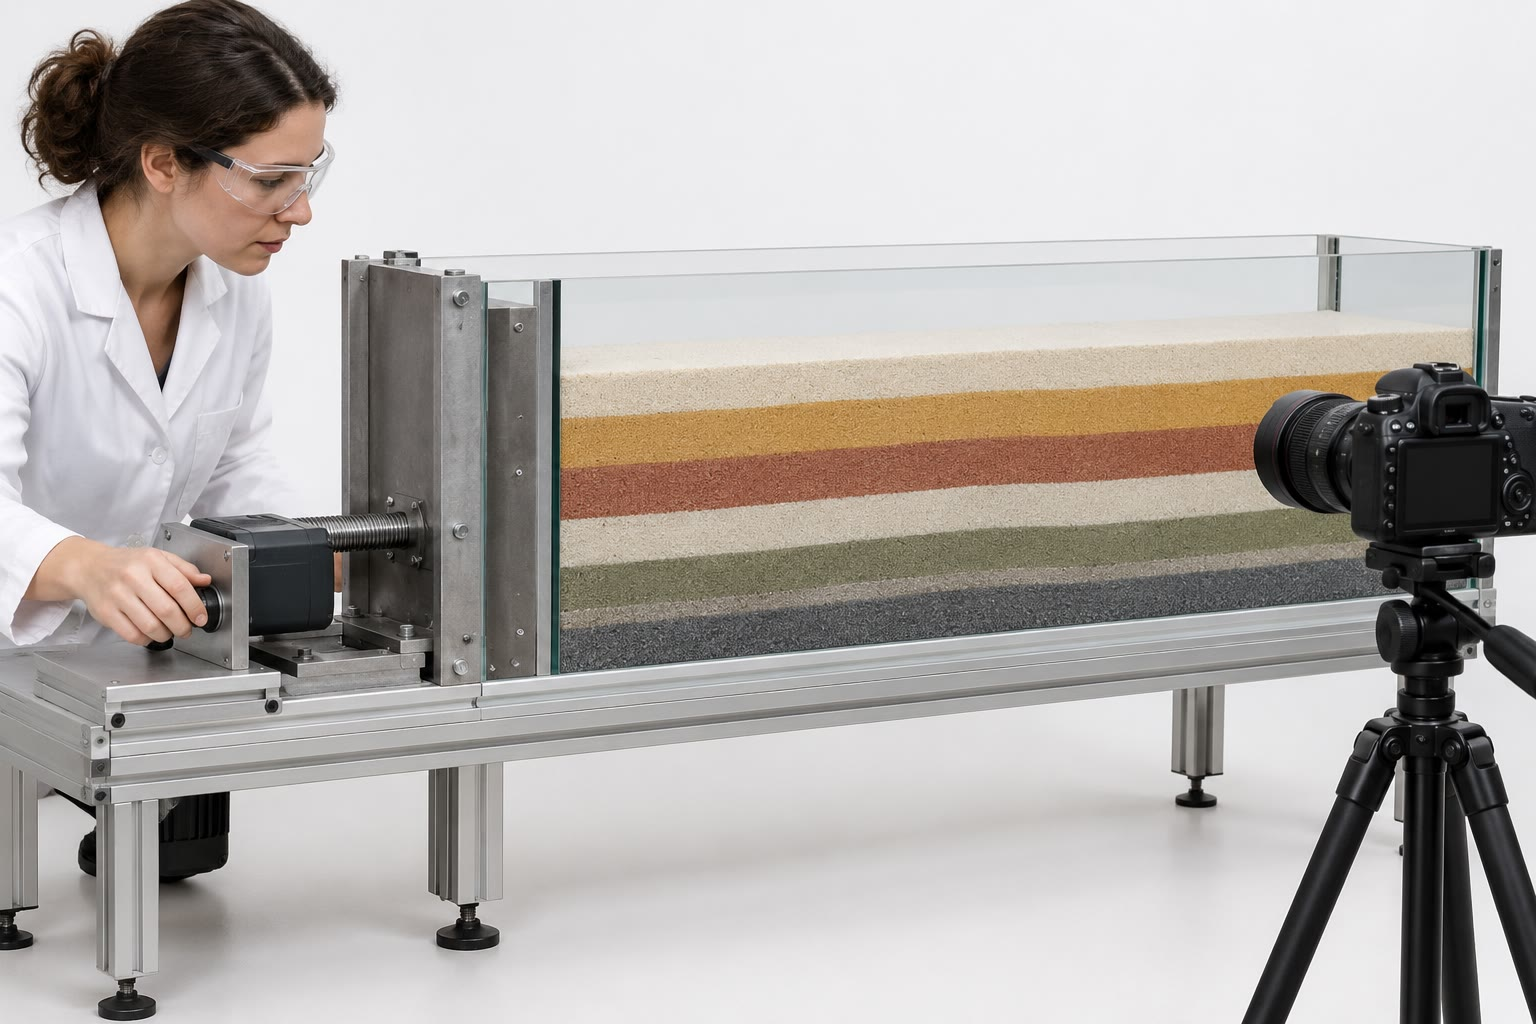
\includegraphics[width=\linewidth]{images/book5/ai/b3-sandbox-lab.jpg}

{\scriptsize Een zandbakmodel vóór verkorting: gekleurde zandlagen in een
bak met glazen wanden, een door een motor aangedreven wand links, een camera op een statief
(Door AI gegenereerde illustratie.)}
\end{minipage}
\end{inthelab}
% ledger: dsd83:taper

\section{Echte wiggen}\label{sec:b3:orogenic-wedges:real}

In de actieve plooi- en overschuivingsgordel van westelijk Taiwan zijn de oppervlaktehelling, de
helling van het décollement en de porendrukken allemaal bekend, uit topografie,
seismische doorsneden en boringen. Davis, Suppe en Dahlen gebruikten ze om de
\omterm{thm:b3:orogenic-wedges:critical-taper}{vergelijking van de kritische wighoek} op te lossen voor de sterkte van de wig en vonden $\mu = 1.03$
binnenin en $\mu_b = 0.85$ aan de basis: de wrijving van Byerlee op de basis, en een
wig die sterker is dan zijn eigen breuken, omdat ze niet allemaal georiënteerd zijn om
gemakkelijk te schuiven. Met deze twee coëfficiënten zetten ze de waargenomen wighoeken van andere
actieve wiggen, op het land en onder zee, om in porendrukverhoudingen, en vonden
ze overal boven hydrostatisch, in lijn met boringen. Ze vonden ook
waar de theorie ophoudt: de wighoek daalt abrupt waar wiggen dikker worden
dan ongeveer \qty{15}{km}, de diepte waarop kwartsrijke gesteenten plastisch worden
bij gebruikelijke geothermen, en de basis gehoorzaamt niet langer aan een wrijvingswet.
% ledger: dsd83:taper

Aan het front van de westelijke Alpen is de Jura een overschuivingswig met een smalle
hoek van slechts 3 tot \ang{4}. Het décollement ligt grotendeels in halietrijke
lagen van Triassische ouderdom, en de vloeistoffen daar zijn niet overdrukt: de
zwakte van zout alleen verklaart de smalle wighoek. Ten zuiden van de Jura, waar de
Triassische lagen geen halliet bevatten, heeft hetzelfde front een wighoek van 12 tot
\ang{13}, met stapels overschuivingsschijven, hoewel de daar gemeten vloeistofdrukken
hoog zijn. In de Centrale Alpen levert de analyse van de \omterm{def:b3:orogenic-wedges:critical-taper}{kritische wighoek} op de
oppervlaktehelling een basale sterkte $\mu_b(1 - \lambda_b)$ (met een kleine
cohesieterm) onder 0.1, en zelfs 0.05 in evaporieten en schalies nabij het front,
die toeneemt richting het achterland, met porendrukverhoudingen boven 0.54. De
basis van een wig is vaak veel zwakker dan de wet van Byerlee zou aangeven, door zijn
gesteentetype en door zijn vloeistoffen.
% ledger: deville21:jura, vonhagke14:alps

\section{Flux door een wig}\label{sec:b3:orogenic-wedges:flux}

Een wig bij zijn \omterm{def:b3:orogenic-wedges:critical-taper}{kritische wighoek} groeit door accretie, bij vaste vorm: zijn lengte
en hoogte nemen samen toe. Erosie verwijdert gesteente van het oppervlak. Wanneer de
twee elkaar in evenwicht houden, behoudt de wig zijn omvang, en stroomt er gesteente door de wig.

\begin{proposition}[Balans van de flux in stationaire toestand]\label{prop:b3:orogenic-wedges:flux}
Een wig met breedte $W$ langs de transportrichting ontvangt, per eenheid van lengte
van de gordel, de accretieflux $F_a = v h$, waarbij $v$ de convergentiesnelheid is
en $h$ de dikte van de inkomende laag boven het décollement. Ze verliest
de erosieflux $F_e = \bar e W$, waarbij $\bar e$ de gemiddelde
erosiesnelheid over het oppervlak is. Haar dwarsdoorsnede verandert met de snelheid $F_a -
F_e$; in stationaire toestand geldt $\bar e = vh/W$.
\end{proposition}

\begin{proof}
In de tijdseenheid passeert een lengte $v$ van de inkomende laag, met dikte $h$,
over zijn teen de wig in, en de dikte $e(x)$ wordt op elk
punt van zijn oppervlak verwijderd; de oppervlakte blijft behouden, dus verandert de oppervlakte van de doorsnede
met $vh - \int_0^W e\,\mathrm dx = F_a - F_e$. In stationaire toestand is de
verandering nul.
\end{proof}

Met $v = \qty{10}{mm/yr}$, $h = \qty{4}{km}$ en $W = \qty{60}{km}$ is de
erosiesnelheid die voor de stationaire toestand nodig is $\qty{0.67}{mm/yr}$. Exhumatie in de
zin van Boek~4 is het verwijderen van het gesteente boven een bepaald gesteente:
in stationaire toestand bereiken gesteenten het oppervlak met de snelheid waarmee erosie
het verlaagt, en de wig brengt ze omhoog vanuit diepten waar ze heet waren. Meten
hoe snel dat gaat, vereist een klok die begint bij een bekende temperatuur.

\section{Thermochronologie}\label{sec:b3:orogenic-wedges:thermochronology}

\begin{definition}[Thermochronologie, thermochronometer]\label{def:b3:orogenic-wedges:thermochronology}
\emph{Thermochronologie}\index{thermochronologie} is het gebruik van radiometrische
afkoelingsouderdommen om het tijdstip te dateren waarop een gesteente een bepaalde
temperatuur passeerde, en zo de thermische geschiedenis ervan te reconstrueren. Een
\emph{thermochronometer}\index{thermochronometer} is een combinatie van een mineraal en
een dateringsmethode met de bijbehorende sluitingstemperatuur: bijvoorbeeld apatiet met de
(U--Th)/He-methode, of zirkoon met fissiesporen.
\end{definition}

De onderstaande tabel ordent de belangrijkste \omterm{def:b3:orogenic-wedges:thermochronology}{thermochronometers} naar sluitingstemperatuur;
de dieptes gaan uit van een gemiddelde oppervlaktetemperatuur van \qty{10}{\celsius} en een
uniforme gradiënt van \qty{30}{\celsius/km}. Een gesteente dat afkoelt terwijl het
wordt geëxhumeerd, passeert ze achtereenvolgens, en de ouderdommen nemen toe van de
methoden met lage temperatuur naar die met hoge temperatuur. De fysica van fissiesporen en van
heliumdiffusie, die deze temperaturen bepaalt, staat
in \cref{ch:b3:advanced-geochronology}.
\begin{center}
\small
% ledger: sueoka19:closure
\begin{tabular}{lcc}
\hline
\omterm{def:b3:orogenic-wedges:thermochronology}{thermochronometer} & sluitingstemperatuur (\unit{\celsius}) & diepte (\unit{km}) \\
\hline
apatiet (U--Th)/He & 50--80 & 1.3--2.3 \\
apatiet fissiesporen & 90--120 & 2.7--3.7 \\
zirkoon (U--Th)/He & 160--200 & 5.0--6.3 \\
zirkoon fissiesporen & ongeveer 280 & 9 \\
\textsuperscript{40}Ar/\textsuperscript{39}Ar op biotiet & 350--400 & 11--13 \\
\textsuperscript{40}Ar/\textsuperscript{39}Ar op muskoviet & ongeveer 425 & 14 \\
U--Pb op zirkoon & boven 900 & --- \\
\hline
\end{tabular}
\end{center}

Deze dieptes zijn slechts een eerste schatting, omdat erosie de geotherm verandert.

\begin{proposition}[Geotherm in stationaire toestand met erosie]\label{prop:b3:orogenic-wedges:geotherm}
Laat gesteente met de constante snelheid $v$ opstijgen door een laag met dikte $L$ waarvan
het oppervlak ($z = 0$) op $T_s$ wordt gehouden en de basis op $T_L$, zonder
warmteproductie. De stationaire temperatuur is
\[
  T(z) = T_s + (T_L - T_s)\,\frac{1 - e^{-\mathrm{Pe}\,z/L}}{1 - e^{-\mathrm{Pe}}},
  \qquad \mathrm{Pe} = \frac{vL}{\kappa},
\]
en de gradiënt aan het oppervlak is $\mathrm{Pe}/(1 - e^{-\mathrm{Pe}})$ maal
de conductieve gradiënt $(T_L - T_s)/L$.
\end{proposition}

\begin{proof}
Een gesteentedeeltje op de diepte $z$ beweegt omhoog, naar kleinere $z$: de
temperatuur die het meedraagt verandert als $\partial T/\partial t - v\,\partial
T/\partial z$, en de diffusievergelijking wordt $\partial T/\partial t - v
T' = \kappa T''$. In stationaire toestand geldt $T'' = -(v/\kappa)T'$, dus $T' = C
e^{-vz/\kappa}$ en $T = T_s + C(\kappa/v)(1 - e^{-vz/\kappa})$, wat voldoet aan
$T(0) = T_s$. Het invullen van $T(L) = T_L$ legt $C$ vast en geeft de formule. Bij $z =
0$ geldt $T' = (T_L - T_s)(\mathrm{Pe}/L)/(1 - e^{-\mathrm{Pe}})$.
\end{proof}

Voor $\mathrm{Pe} \ll 1$ nadert de factor 1: conductie wint en de
geotherm blijft recht. Voor $v = \qty{1}{mm/yr}$ over \qty{30}{km}, met
$\kappa = \qty{e-6}{m^2/s}$, $\mathrm{Pe} = 0.95$ en de gradiënt aan het oppervlak
stijgt van 30 naar \qty{46}{\celsius/km}: de isothermen drukken naar het
oppervlak en elke \omterm{def:b3:orogenic-wedges:thermochronology}{thermochronometer} sluit op een ondiepere diepte.
% ledger: england:kelvin, earle:settings

\begin{definition}[Ouderdom--hoogterelatie]\label{def:b3:orogenic-wedges:age-elevation}
De \emph{ouderdom--hoogterelatie}\index{ouderdom--hoogterelatie} van een
\omterm{def:b3:orogenic-wedges:thermochronology}{thermochronometer} is de grafiek van de afkoelingsouderdommen van monsters die over een
reeks hoogten zijn verzameld, meestal langs een steile helling of een verticaal profiel,
uitgezet tegen hun hoogten.
\end{definition}

\begin{proposition}[Helling van de ouderdom--hoogterelatie]\label{prop:b3:orogenic-wedges:age-elevation}
Laat gesteenten verticaal opstijgen met de constante snelheid $v$ onder een stationaire
topografie, en laat de sluitingsisotherm op de hoogte $e(x) = e_0 +
f\,h(x)$ liggen, waarbij $h(x)$ de hoogte van het oppervlak is en $0 \le f < 1$. Een monster
dat aan het oppervlak op hoogte $h$ is verzameld, heeft de ouderdom $t = (h - e)/v$,
en de \omterm{def:b3:orogenic-wedges:age-elevation}{ouderdom--hoogterelatie} is een rechte lijn met helling
\[
  \frac{\mathrm dh}{\mathrm dt} = \frac{v}{1 - f}.
\]
Bij een vlakke isotherm is $f = 0$ en is de helling de exhumatiesnelheid.
\end{proposition}

\begin{proof}
Het gesteente dat nu aan het oppervlak bij $x$ ligt, passeerde de sluitingsisotherm recht
eronder, op hoogte $e(x)$, en is sindsdien $h - e$ gestegen, met snelheid $v$:
$t = (h - e_0 - fh)/v = ((1 - f)h - e_0)/v$. Hieruit volgt $\mathrm dt/\mathrm dh =
(1 - f)/v$.
\end{proof}

\begin{omfigure}
\begin{tikzpicture}
\begin{groupplot}[group style={group size=2 by 1, horizontal sep=1.7cm},
  omrecord, width=0.47\linewidth, height=0.45\linewidth, title style={font=\small},
  legend style={font=\scriptsize, legend cell align=left}]
\nextgroupplot[title={(a) ouderdom--hoogte}, xlabel={(U--Th)/He-ouderdom van apatiet (\unit{Myr})},
  ylabel={hoogte boven het gemiddelde (\unit{km})}, xmode=log, xmin=0.1, xmax=10,
  log ticks with fixed point, xtick={0.1,0.2,0.5,1,2,5,10}, ymin=-1, ymax=1]
% computed in figdata/bachelor-3/age_elevation.py
\addplot[black, thick, densely dotted] table[x=a30, y=h] {figdata/out/bachelor-3-age_elevation-ages.dat};
\addplot[red!70!black, thick, densely dashed] table[x=a10, y=h] {figdata/out/bachelor-3-age_elevation-ages.dat};
\addplot[omDef, thick] table[x=a03, y=h] {figdata/out/bachelor-3-age_elevation-ages.dat};
\nextgroupplot[title={(b) de sluitingsisotherm}, xlabel={afstand (\unit{km})},
  ylabel={hoogte boven het gemiddelde (\unit{km})}, xmin=0, xmax=40, ymin=-3.3, ymax=1.2,
  legend style={at={(0.5,0.03)}, anchor=south, legend columns=2}]
\addplot[black!70, very thick] table[x=x, y=h] {figdata/out/bachelor-3-age_elevation-iso.dat};
\addlegendentry{oppervlak}
\addplot[black, thick, densely dotted] table[x=x, y=e30] {figdata/out/bachelor-3-age_elevation-iso.dat};
\addlegendentry{\qty{3}{mm/yr}}
\addplot[red!70!black, thick, densely dashed] table[x=x, y=e10] {figdata/out/bachelor-3-age_elevation-iso.dat};
\addlegendentry{\qty{1}{mm/yr}}
\addplot[omDef, thick] table[x=x, y=e03] {figdata/out/bachelor-3-age_elevation-iso.dat};
\addlegendentry{\qty{0.3}{mm/yr}}
\end{groupplot}
\end{tikzpicture}

\par\smallskip{\small Stationaire exhumatie onder een sinusvormig reliëf met
golflengte \qty{20}{km} en amplitude \qty{1}{km}, bij drie snelheden,
lijnstijlen zoals in de legenda van (b) (model van de eerste orde; laag \qty{30}{km} dik, oppervlak op \qty{10}{\celsius},
\qty{30}{\celsius/km} zonder erosie, $\kappa = \qty{e-6}{m^2/s}$, verticale
temperatuurgradiënt van de atmosfeer \qty{6.5}{\celsius/km}, sluiting bij \qty{65}{\celsius}). (a) Ouderdom tegen
hoogte: de hellingen zijn 0.59, 2.5 en \qty{14}{mm/yr}, niet 0.3, 1 en 3.
(b) De \qty{65}{\celsius}-isotherm volgt de topografie nauwkeuriger naarmate de
exhumatie sneller verloopt, omdat hij dichter bij het oppervlak komt.}\label{fig:b3:orogenic-wedges:age-elevation}
\end{omfigure}
% ledger: earle:settings, england:kelvin, ussa76:layers, sueoka19:closure

Isothermen liggen onder een reliëf niet vlak: het oppervlak is op de toppen
kouder dan in de dalen, met de atmosferische temperatuurgradiënt, maar veel minder dan
het gesteente op dezelfde hoogte ondergronds zou zijn, en de ondiepe isothermen
volgen de topografie op een gedempte manier. Voor een sinusvormige topografie met
golflengte $\Lambda$ en een atmosferische temperatuurgradiënt $\Gamma$ levert een oplossing van de eerste orde van de
stationaire vergelijking op:
\[
  f = \frac{(G_0 - \Gamma)\,e^{-mz_c}}{G(z_c)},\qquad
  m = \frac{v}{2\kappa} + \sqrt{\Bigl(\frac{v}{2\kappa}\Bigr)^2 +
  \Bigl(\frac{2\pi}{\Lambda}\Bigr)^2},
\]
waarin $z_c$ de diepte van de sluitingsisotherm onder het gemiddelde oppervlak is,
$G_0$ de oppervlaktegradiënt en $G(z_c)$ de gradiënt op $z_c$ (aangenomen;
het script toetst dit). De storing neemt met de diepte af over de
afstand $1/m$, hooguit $\Lambda/2\pi$: \omterm{def:b3:orogenic-wedges:thermochronology}{thermochronometers} met een lage sluitingstemperatuur,
die ondiep sluiten, voelen het reliëf het sterkst. De figuur hierboven toont het effect
voor apatiet (U--Th)/He.
% ledger: sueoka19:closure, ussa76:layers

Een ouderdom--hoogteprofiel meet de exhumatiesnelheid alleen waar de
sluitingsisotherm onder het reliëf vlak is. Elders overschat het de snelheid met de factor $1/(1 - f)$, die voor apatiet (U--Th)/He bij een reliëf
met een golflengte van \qty{20}{km} tot twee of meer oploopt.
Ouderdommen van meerdere \omterm{def:b3:orogenic-wedges:thermochronology}{thermochronometers} aan dezelfde monsters en thermische modellen
van het reliëf corrigeren hiervoor.

\section{Oefeningen}

\begin{exercise}[$\star$]\label{exo:b3:orogenic-wedges:1}
Bereken $K$ en de verhouding $\sigma'_1/\sigma'_3$ bij bezwijking voor een wig met
$\phi = \ang{30}$.
\end{exercise}

\begin{exercise}[$\star$]\label{exo:b3:orogenic-wedges:2}
Een zandbakwig van droog zand ($\lambda = \lambda_b = 0$) heeft $\mu = 0.6$
binnenin en $\mu_b = 0.3$ aan de basis. Bereken de kritische oppervlaktehelling op een
horizontale basis, en vervolgens op een basis die \ang{3} helt.
\end{exercise}

\begin{exercise}[$\star$]\label{exo:b3:orogenic-wedges:3}
Controleer bij een oppervlak op \qty{10}{\celsius} en een gradiënt van \qty{30}{\celsius/km},
de dieptes uit de tabel met sluitingstemperaturen voor apatiet
(U--Th)/He, apatiet-sporenfissie en zirkoon-sporenfissie. Welke
\omterm{def:b3:orogenic-wedges:thermochronology}{thermochronometer} is het geschiktst om exhumatie vanaf \qty{5}{km} te dateren?
\end{exercise}

\begin{exercise}[$\star$]\label{exo:b3:orogenic-wedges:4}
Een ramp van \qty{2}{km} hoog helt \ang{30}. Bereken de horizontale lengte en de
lengte langs de helling. Hoeveel wordt een laag van de hangende wand opgetild nadat
hij de hele ramp is gepasseerd, en welke verschuiving brengt de snijlijn van de onderste
laag van de voet van de ramp naar de bovenste flat?
\end{exercise}

\begin{exercise}[$\star\star$]\label{exo:b3:orogenic-wedges:5}
Bereken met de Taiwan-coëfficiënten de kritische oppervlaktehelling op een basis
die \ang{6} helt voor $\lambda = \lambda_b = 0.4$ en $0.9$. Wat doet een
toename van de vloeistofdruk met een wig die op zijn \omterm{def:b3:orogenic-wedges:critical-taper}{kritische wighoek} stond?
\end{exercise}

\begin{exercise}[$\star\star$]\label{exo:b3:orogenic-wedges:6}
Een \omterm{def:b3:orogenic-wedges:thrust-folds}{breukbuigplooi} ligt boven een ramp van \qty{1.5}{km} hoog; een laag boven de
bovenste flat vertoont een overschot aan oppervlak van \qty{6.0}{km^2}. Bereken de verschuiving. Een collega
leest dezelfde plooi als een \omterm{def:b3:orogenic-wedges:thrust-folds}{onthechtingsplooi}, waarbij de laag \qty{3.0}{km} boven
het décollement ligt. Welke verkorting zou hij vinden?
\end{exercise}

\begin{exercise}[$\star\star$]\label{exo:b3:orogenic-wedges:7}
Neem $\mu = 0.6$ binnenin zowel de Jura-wig (wighoek \ang{3.5}) als de wig ten
zuiden ervan (wighoek \ang{12.5}), een hydrostatische $\lambda = 0.4$ binnenin beide, en een
basishelling van \ang{2} voor beide. Bereken de basissterkte $\mu_b(1 -
\lambda_b)$ die elke wighoek vereist, en vergelijk die met Byerlee's $0.85$
bij hydrostatische druk. Is het resultaat in overeenstemming met het décollement in
halliet onder de Jura?
\end{exercise}

\begin{exercise}[$\star\star$]\label{exo:b3:orogenic-wedges:8}
Gesteente stijgt met \qty{1}{mm/yr} door een laag van \qty{30}{km} dik, van
\qty{910}{\celsius} aan de basis tot \qty{10}{\celsius} aan het oppervlak, met
$\kappa = \qty{e-6}{m^2/s}$. Bereken het thermisch Pécletgetal, de oppervlaktegradiënt,
en de diepte van de \qty{65}{\celsius}-isotherm. Vergelijk met de diepte
zonder erosie.
\end{exercise}

\begin{exercise}[$\star\star$]\label{exo:b3:orogenic-wedges:9}
Twee monsters van dezelfde helling, op 1200 en \qty{2000}{m}, hebben apatiet
(U--Th)/He-ouderdommen van 3.4 en \qty{4.6}{Myr}. Bereken de schijnbare
exhumatiesnelheid. Een thermisch model van het reliëf geeft $f = 0.5$: wat is de werkelijke snelheid?
\end{exercise}

\begin{exercise}[$\star\star\star$]\label{exo:b3:orogenic-wedges:10}
Toon aan dat voor $\lambda = \lambda_b$ de kritische oppervlaktehelling verdwijnt bij een
basishelling $\beta^* = \mu_b/K$ die niet van $\lambda$ afhangt. Bereken deze voor
Taiwan. Wat gebeurt er met een wig waarvan de basis steiler helt?
\end{exercise}

\begin{exercise}[$\star\star\star$]\label{exo:b3:orogenic-wedges:11}
Toon aan dat voor een zeer lange golflengte en een zeer trage exhumatie $f$ naar
$1 - \Gamma/G$ neigt, waarbij $G$ de uniforme gradiënt is; evalueer het voor $G =
\qty{30}{\celsius/km}$ en $\Gamma = \qty{6.5}{\celsius/km}$. Wat is dan de
helling van de \omterm{def:b3:orogenic-wedges:age-elevation}{ouderdom--hoogterelatie}? Neem $v = \qty{1}{mm/yr}$ en de
waarden van oefening~8 ($z_c = \qty{1.21}{km}$, $G_0 = \qty{46.5}{\celsius/km}$,
$G(z_c) = \qty{44.7}{\celsius/km}$) en bereken $f$ voor golflengten van 5 en
\qty{20}{km}.
\end{exercise}

\begin{exercise}[$\star\star\star$]\label{exo:b3:orogenic-wedges:12}
Een wig groeit op zijn \omterm{def:b3:orogenic-wedges:critical-taper}{kritische wighoek} $\alpha + \beta$ uitsluitend door \omterm{def:b3:orogenic-wedges:accretion}{frontale accretie},
zonder erosie, vanuit de flux $F_a$. Toon aan dat de breedte ervan groeit als
$W = \sqrt{2F_at/\tan(\alpha + \beta)}$. Neem $F_a = \qty{40}{km^2/Myr}$ en
een wighoek van \ang{6}. Hoe breed is de wig na \qty{2}{Myr}, en hoe lang duurt het
voordat hij \qty{60}{km} bereikt?
\end{exercise}

\section{Probleem: Het front van de Kestrelwig}

\begin{problem}[{Weekendprobleem --- de verkorting, mechanica, flux en
exhumatie van een verzonnen overschuivingswig}]
\label{pb:b3:orogenic-wedges:1}
% values: calc/ch10.py; critical_taper.py; age_elevation.py; fault_bend.py
De Kestrelketen is het verzonnen front van een bergketen, een bovengronds
plooi-en-overschuivingsgordel van \qty{60}{km} breed, die met \qty{10}{mm/yr} wordt geduwd over een
voorland waarvan de sedimentlaag \qty{4.0}{km} dik is boven een
schalie-décollement. De frontale overschuiving volgt het décollement \qty{4.5}{km} onder
het oppervlak, klimt over een ramp met een helling van \ang{25} en loopt langs een bovenste flat
\qty{1.5}{km} diep. Aan het front staat het oppervlak \qty{0.3}{km} boven zeeniveau
en ligt het décollement \qty{4.0}{km} eronder; \qty{60}{km} achter het front staat het oppervlak
op \qty{2.4}{km} en ligt het décollement
\qty{8.2}{km} onder zeeniveau. Neem, zoals in Taiwan, $\mu = 1.03$ en $\mu_b =
0.85$, een gesteentedichtheid van \qty{2500}{kg/m^3}, water van \qty{1000}{kg/m^3} en
$g = \qty{9.81}{m/s^2}$.

\medskip\noindent\textbf{Deel I --- Geometrie van de overschuiving.}
\begin{enumerate}
  \item Bereken de hoogte van de ramp, de horizontale lengte ervan en de lengte
        langs de helling.
  \item Hoeveel is een laag van de hangende wand omhooggekomen nadat ze
        de hele ramp is gepasseerd?
  \item Boven de ramp vertoont een laag die op de bovenste flat ligt een extra oppervlakte
        van \qty{16.5}{km^2} boven haar regionale niveau. Bereken de verschuiving.
  \item Welke extra oppervlakte voorspelt men voor een ondiepere laag? Had de plooi
        als \omterm{def:b3:orogenic-wedges:thrust-folds}{onthechtingsplooi} over het décollement gelezen moeten worden, met de laag
        \qty{4.0}{km} erboven, welke verkorting zou dan zijn gevonden?
  \item Achter de ramp toont een seismische sectie een duplex van vier paarden, elk
        nu \qty{2.5}{km} lang langs de vloeroverschuiving, gesneden uit plakken van
        \qty{6.0}{km} lengte. Bereken de verkorting die door de paarden is opgenomen, en
        vergelijk die met de verschuiving op de frontale ramp.
  \item De paarden zijn na elkaar gevormd. Welke is de jongste, en waarom is de
        dakoverschuiving geplooid?
\end{enumerate}

\medskip\noindent\textbf{Deel II --- De wighoek.}
\begin{enumerate}[resume]
  \item Bereken de oppervlaktehelling $\alpha$, de basale helling $\beta$ en de
        wighoek.
  \item Bereken de dikte van de wig \qty{60}{km} achter het front. Kan
        de Coulomb-wigtheorie worden gebruikt?
  \item Bereken $K$. Welke oppervlaktehelling zou een droge wig op deze basis hebben?
  \item Welke oppervlaktehelling zou hij hebben bij hydrostatische vloeistofdruk in
        de wig en aan zijn basis? Is de wig daarmee consistent?
  \item Los de \omterm{thm:b3:orogenic-wedges:critical-taper}{vergelijking van de kritische wighoek} op voor $\lambda = \lambda_b$.
  \item Bereken de verticale spanning, de vloeistofdruk en de hydrostatische
        druk aan de basis van de wig \qty{60}{km} achter het front.
  \item Drainage verlaagt $\lambda$ tot 0.7. Bereken de nieuwe kritische
        oppervlaktehelling. Hoe reageert de wig?
\end{enumerate}

\medskip\noindent\textbf{Deel III --- De flux.}
\begin{enumerate}[resume]
  \item Bereken de accretieflux per kilometer van de gordel.
  \item Welke gemiddelde erosiesnelheid houdt de wig in de stationaire toestand?
  \item Bereken het volume en de massa gesteente die per jaar uit
        \qty{100}{km} van de gordel worden geërodeerd.
  \item Als erosie zou stoppen, hoe snel zou de wig dan in eerste instantie verbreden?
  \item Als de helft van de inkomende laag als \omterm{def:b3:orogenic-wedges:accretion}{tektonische underplating} onder het achterste deel
        van de wig terechtkomt in plaats van aan zijn front geaccreteerd, zou de gemiddelde
        erosiesnelheid in de stationaire toestand dan veranderen? Waar zou de erosie zich concentreren?
\end{enumerate}

\medskip\noindent\textbf{Deel IV --- De klok.}
Neem de laag \qty{30}{km} dik, \qty{10}{\celsius} aan het gemiddelde oppervlak
(\qty{2.0}{km} boven zeeniveau) en \qty{910}{\celsius} aan haar basis, $\kappa
= \qty{e-6}{m^2/s}$, een sluitingstemperatuur van \qty{65}{\celsius} voor apatiet
(U--Th)/He, een verticale temperatuurgradiënt van \qty{6.5}{\celsius/km} en een reliëf met
golflengte \qty{20}{km}. Vijf monsters die aan één dalwand zijn verzameld, geven:
\begin{center}
\small
\begin{tabular}{lccccc}
\hline
hoogte (\unit{km}) & 1.30 & 1.65 & 2.00 & 2.35 & 2.70 \\
apatiet (U--Th)/He-ouderdom (\unit{Myr}) & 1.60 & 1.83 & 2.07 & 2.30 & 2.54 \\
\hline
\end{tabular}
\end{center}
\begin{enumerate}[resume]
  \item Neem de erosiesnelheid van vraag 15 als exhumatiesnelheid en bereken
        het \omterm{def:b3:lithosphere-thermal-models:peclet}{thermische Pécletgetal} en de oppervlaktegradiënt.
  \item Bereken de diepte van de sluitingsisotherm onder het gemiddelde oppervlak en
        de gradiënt daar.
  \item Welke ouderdom zou een monster op de gemiddelde hoogte hebben bij een vlakke
        sluitingsisotherm? Vergelijk met de gegevens.
  \item Bereken $m$ en de doorbuigingsfactor $f$.
  \item Pas een rechte lijn aan op de ouderdom--hoogtegegevens. Welke schijnbare
        exhumatiesnelheid geeft de helling?
  \item Corrigeer die voor de doorbuiging van de isotherm.
  \item Vergelijk met Deel III en geef de exhumatiesnelheid van de
        Kestrelwig.
\end{enumerate}
\end{problem}
